\documentclass[aspectratio=169]{beamer}
\usepackage[scale=2.5]{ccicons}
\usepackage{tikz}
   \usetikzlibrary{matrix}

\newcommand{\key}[1]{\texttt{\color{UOWorange}#1}} 
\newcommand{\val}[1]{\texttt{\color{UOWblue}#1}} 
\newcommand{\command}[1]{\texttt{\color{UOWdarkgreen}#1}} 

\title{The Presentation Title}
\subtitle{A nice little subtitle}
\author[Thomas]{Thomas M Griffiths}
\institute{School of Chemistry}
\date{}

\usetheme[]{uow}

\begin{document}

\maketitle

\begin{frame}
   \frametitle{Coelenterazine, Check it!}
   \begin{columns}[T]
      \begin{column}{0.5\textwidth}
         \begin{enumerate}
            \item Imidazopyrazinone backbone (in red).
            \item Most common substrate in \textbf{marine bioluminescence}.
            \item Proposed antioxidant capabilities.
            \item Unknown uptake or synthetic pathway in nature.
            \item $y=mx+b$ is some example mathematics.
         \end{enumerate}
      \end{column}
      \begin{column}{0.5\textwidth}
         \centering
         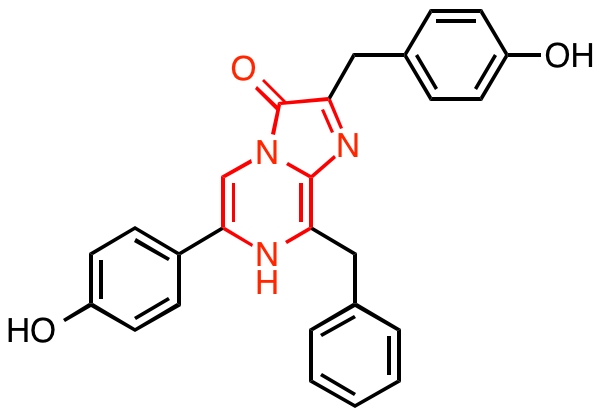
\includegraphics[width=\textwidth]{coelenterazine.png}
      \end{column}
   \end{columns}
\end{frame}

\begin{frame}[fragile]
\frametitle{Typography}
\begin{verbatim}
The theme provides sensible defaults to 
\emph{emphasize} text, \alert{accent} parts 
or show \textbf{bold} results.
\end{verbatim}
\begin{center} \textit{becomes} \end{center}
The theme provides sensible defaults to \emph{emphasize} text, \alert{accent} parts or show \textbf{bold} results.
\end{frame}


%\begin{frame}{The UOW colour palette}
%\centering
%\begin{tikzpicture}[ampersand replacement=\&, every node/.style={anchor=west}]
%\scriptsize
%\matrix (m) [row sep=0.25em, column sep=3em, nodes={align=left}] {%
%   \node[align=left] {\textbf{Key Value}}; \& %
%   \node[align=left] {\textbf{Colour Name}};   \& %
%   \node[align=left] {\textbf{RGB Tuple}};   
%   \& \draw [line width=0.4pt, color=UOWblack] (0,0)  circle (0.7em); \\ %
%   \node[align=left] {\val{black}};     \& \node[align=left] {UOWblack};     \& \node {0, 0, 0};      %
%   \& \fill [line width=1em, color=UOWblack] (0,0)  circle (0.7em); \\
%   \node[align=left] {\val{grey}};      \& \node[align=left] {UOWgrey};      \& \node {69, 85, 95};   %
%   \& \fill [line width=1em, color=UOWgrey] (0,0)  circle (0.7em); \\
%   \node[align=left] {\val{darkred}};   \& \node[align=left] {UOWdarkred};   \& \node {195, 18, 48};  %
%   \& \fill [line width=1em, color=UOWdarkred] (0,0)  circle (0.7em); \\
%   \node[align=left] {\val{red}};       \& \node[align=left] {UOWred};       \& \node {238, 64, 52};  %
%   \& \fill [line width=1em, color=UOWred] (0,0)  circle (0.7em); \\
%   \node[align=left] {\val{pink}};      \& \node[align=left] {UOWpink};      \& \node {238 ,0, 139};  %
%   \& \fill [line width=1em, color=UOWpink] (0,0)  circle (0.7em); \\
%   \node[align=left] {\val{orange}};    \& \node[align=left] {UOWorange};    \& \node {243, 121, 32}; %
%   \& \fill [line width=1em, color=UOWorange] (0,0)  circle (0.7em); \\
%   \node[align=left] {\val{gold}};      \& \node[align=left] {UOWgold};      \& \node {253, 184, 19}; %
%   \& \fill [line width=1em, color=UOWgold] (0,0)  circle (0.7em); \\
%   \node[align=left] {\val{limegreen}}; \& \node[align=left] {UOWlimegreen}; \& \node {183, 198, 38}; %
%   \& \fill [line width=1em, color=UOWlimegreen] (0,0)  circle (0.7em); \\
%   \node[align=left] {\val{darkgreen}}; \& \node[align=left] {UOWdarkgreen}; \& \node {0, 146, 94};   %
%   \& \fill [line width=1em, color=UOWdarkgreen] (0,0)  circle (0.7em); \\
%   \node[align=left] {\val{blue}};      \& \node[align=left] {UOWblue};      \& \node {0, 149, 214};  %
%   \& \fill [line width=1em, color=UOWblue] (0,0)  circle (0.7em); \\
%   \node[align=left] {\val{darkblue}};  \& \node[align=left] {UOWdarkblue};  \& \node {0, 83, 154};   %
%   \& \fill [line width=1em, color=UOWdarkblue] (0,0)  circle (0.7em); \\
%   \node[align=left] {\val{purple}};    \& \node[align=left] {UOWpurple};    \& \node {74, 47, 142};  %
%   \& \fill [line width=1em, color=UOWpurple] (0,0)  circle (0.7em); \\
%};
%\end{tikzpicture}
%\vspace*{1em}
%\end{frame}
%
%
%\begin{frame} 
%\frametitle{There Is No Largest Prime Number} 
%\begin{theorem}
%There is no largest prime number. 
%\end{theorem} 
%\begin{enumerate} 
%\item Suppose $p$ were the largest prime number. 
%\item Let $q$ be the product of the first $p$ numbers.\footnote{An example footnote.}
%\item Then $q+1$ is not divisible by any of them. 
%\item But $q + 1$ is greater than $1$, thus divisible by some prime number not in the first $p$ numbers.\footnote{A second example footnote.}
%\end{enumerate}
%\end{frame}
%
%
%\begin{frame}{Itemised Lists With Columns}
%   \begin{columns}[T]
%      \begin{column}{0.48\textwidth}
%      Lorem ipsum dolor sit amet, consetetur sadipscing elitr, sed diam nonumy eirmod tempor invidunt ut labore et dolore magna aliquyam erat, sed diam voluptua. At vero eos et accusam et justo duo dolores et ea rebum. Stet clita kasd gubergren, no sea takimata sanctus est Lorem ipsum dolor sit amet. Lorem ipsum dolor sit amet, consetetur sadipscing elitr, sed diam nonumy eirmod tempor.
%      \end{column}
%      \begin{column}{0.48\textwidth}
%      \begin{itemize}
%         \item One point
%         \item Another point
%         \item And a \alert{third}!
%      \end{itemize}
%      \end{column}
%   \end{columns}
%\end{frame}
%
%
%\begin{frame}
%   \begin{block}{Observation 2}
%   Simmons Dormitory is composed of brick.
%   \end{block}
%\end{frame}
%
%
%\begin{frame}
%   \begin{alertblock}{Observation 2}
%   Simmons Dormitory is composed of brick.
%   \end{alertblock}
%\end{frame}
%
%
%\begin{frame}
%   \begin{exampleblock}{Observation 2}
%   Simmons Dormitory is composed of brick.
%   \end{exampleblock}
%\end{frame}
%
%
%\begin{frame}\footnotesize
%   The Beamer implementation 'UOWtheme' is copyright (CC BY-NC-SA 4.0 Int) 2015 by T. M. Griffiths under the \href{http://creativecommons.org/licenses/by-sa/4.0/}{Creative Commons Attribution-Share Alike 4.0 International License}\footnote{\url{http://creativecommons.org/licenses/by-nc-sa/4.0/}}.
%   
%   \begin{center}\ccbysa\end{center}
%   
%   The crest and associated branding of the University of Wollongong is copyright and the property of the University of Wollongong. As the core identifier of the university its use is governed by the university's brand and visual identity guidelines which can be found \href{http://www.uow.edu.au/about/brand/uowlogo/index.html}{online}\footnote{\url{http://www.uow.edu.au/about/brand/uowlogo/index.html}}.
%   
%\end{frame}

\end{document}
